\documentclass[letterpaper]{article}

\usepackage{cite}
\usepackage[utf8]{inputenc}
\usepackage{graphicx}
\usepackage{hyperref}
\usepackage{amsmath,amsthm,amssymb,mathtools}
\usepackage{prftree}

\usepackage{tikz}
\usetikzlibrary{calc,positioning,fit,shapes}

\newcommand{\todo}[1]{{\color{red}[TODO: #1]}}

\begin{document}

\section{Language Design}

The language has the following design goals:

\begin{itemize}
\item A useful foundational set of parser primitives and combinators,
\item A capacity to capture context-sensitivity and data-dependency
  via a constraint system, and
\item  A module system that enables nested grammars and composes with
  the constraint system.
\end{itemize}

\begin{itemize}
\item The core structure of a Parsley specification is provided by a
  {\em parsing expression grammar (PEG)} \cite{ford2004popl},
  specified in notation similar to  {\em extended BNF (EBNF)} for
  grammar productions.  Although {\em context-free grammars (CFGs)}
  use the EBNF notation, there are critical differences in the PEG
  notation: (a) the choice combinator in PEGs is ordered, as opposed
  to non-deterministic in CFGs, and (b) the PEG notation includes
  syntactic predicates that do not occur in CFGs.  The choice of a PEG
  core provides us the set of primitives and combinators as we desire.

\item Context management is provided by a fairly traditional
  attribute-grammar system, where the expression language for
  attribute computations is purely functional and strongly-typed.  In
  Parsley, non-terminals have user-defined attributes, while terminals
  have a default attribute value of type byte or byte-string.  This
  provides us with the tools needed to capture context-sensitivity.

\item Additional context-sensitivity is provided by a constraint
  system that guards further processing  within a non-terminal production.
  The constraint language uses the attribute system to perform
  context-sensitive checks, and employs primitives in the constraint
  expression language to perform data-dependent parsing.

\item A module system allows the composition of independent grammars.
\end{itemize}

The expression sublanguage used in attribute updates and constraints
is a strongly typed polymorphic functional language supporting
user-defined types and functions.  It includes a standard library of
common types and utility functions.  The expression and data type
sublanguage is designed to ensure that recursive and iterative
computations always terminate.

\section{Language Use}

\begin{figure*}[!ht]
  \centering
  \resizebox{10cm}{!}{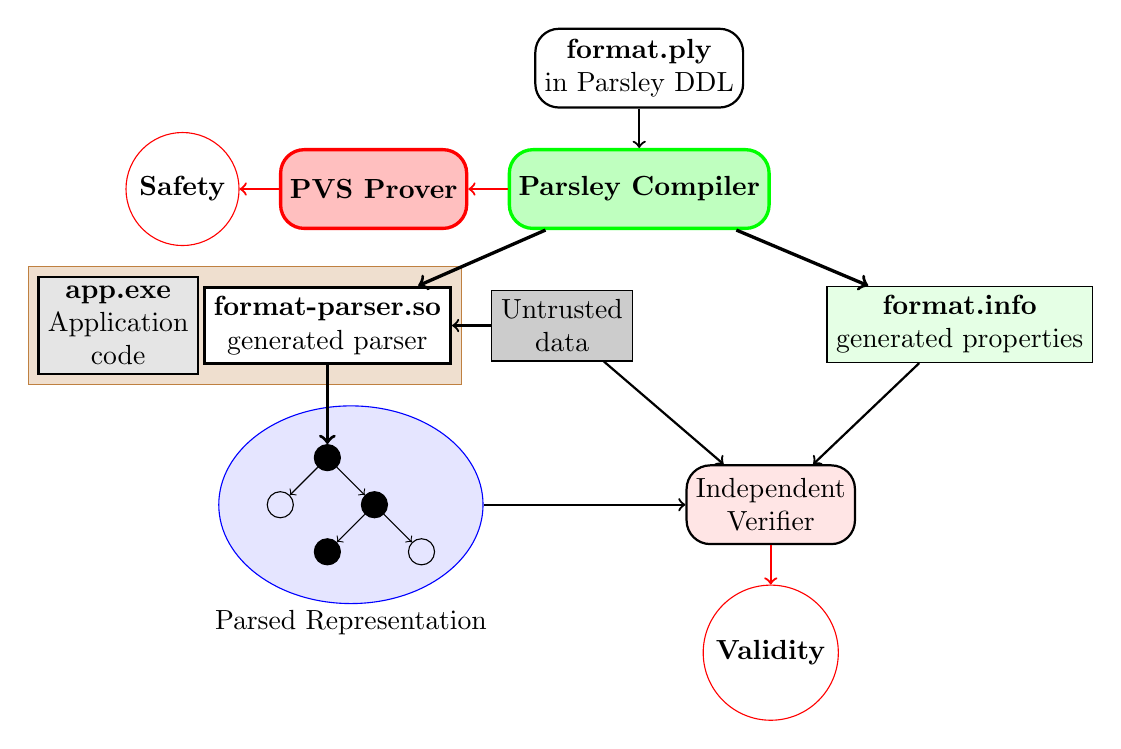
\begin{tikzpicture}[
    node distance=5mm,
    align=center,
    spec/.style={rectangle, rounded corners=3mm, minimum size=10mm, draw=black, thick},
    info/.style={rectangle, draw=black, fill=green!10!white},
    lib/.style={rectangle, very thick, draw=black, fill=white},
    app/.style={rectangle, thick, draw=black, fill=black!10!white},
    prog/.style={rectangle, draw=brown, fill=brown!25!white},
    compiler/.style={rectangle, rounded corners=3mm, minimum size=10mm,
      very thick, draw=green, fill=green!25!white},
    prover/.style={rectangle, rounded corners=3mm, minimum size=10mm,
      very thick, draw=red, fill=red!25!white},
    verifier/.style={rectangle, rounded corners=3mm, minimum size=10mm,
      thick, draw=black, fill=red!10!white},
    data/.style={rectangle, draw=black, fill=black!20!white},
    prop/.style={circle, draw=red},
    ast/.style={circle, draw=black},
    memory/.style={ellipse, draw=blue, fill=blue!10!white},
    input/.style={->, thick, black},
    gen/.style={->, very thick, black},
    proverinput/.style={->, thick, red},
    proveroutput/.style={->, thick, red},
    tree/.style={->, black},
  ]

  \pgfdeclarelayer{background}
  \pgfdeclarelayer{main}
  \pgfdeclarelayer{foreground}
  \pgfsetlayers{background,main,foreground}

  % main pipeline
  \begin{pgfonlayer}{main}
    \node (spec)      [spec]                         {\textbf{format.ply}\\ in Parsley DDL};

    \node (compiler)  [compiler, below=of spec]      {\textbf{Parsley Compiler}};

    \node (prover)    [prover, left=of compiler]     {\textbf{PVS Prover}};

    \node (safety)    [prop,left=of prover]          {\textbf{Safety}};

    \node (lib)       [lib, below left=1cm of compiler]   {\textbf{format-parser.so}\\ generated parser};

    \node (info)      [info, below right=1cm of compiler] {\textbf{format.info}\\ generated properties};

    \node (app)       [app, left=0.5mm of lib]       {\textbf{app.exe}\\ Application\\ code};

    \node (data)      [data, right=of lib]           {Untrusted\\ data};
  \end{pgfonlayer}

  % complete application
  \begin{pgfonlayer}{background}
    \node (prog)      [prog, fit=(app.south west) (app.north west)
                                 (lib.south east) (lib.north east)] {};
  \end{pgfonlayer}

  % generated AST in memory
  \begin{pgfonlayer}{main}
    \node (root)      [ast, fill=black, below] at ($(lib.south)+(0,-1cm)$)  {};

    \node (c0)        [ast, below left=of root] {};
    \node (c1)        [ast, below right=of root, fill=black] {};
    \node (c10)       [ast, below left=of c1, fill=black] {};
    \node (c11)       [ast, below right=of c1] {};
  \end{pgfonlayer}
  \begin{pgfonlayer}{background}
    \node (tree)      [memory, fit=(root) (c0) (c1) (c10) (c11)] {};
  \end{pgfonlayer}

  \begin{pgfonlayer}{main}
    \node (appdata)   [below=-0.5mm of tree] {Parsed Representation};
    \node (verifier)  [verifier] at (compiler.south east |- tree) {Independent\\Verifier};
    \node (validity)  [prop, below=of verifier] {\textbf{Validity}};
  \end{pgfonlayer}

  % flow
  \draw[input]         (spec) -- (compiler);
  \draw[gen]           (compiler) -- (lib);
  \draw[gen]           (compiler) -- (info);
  \draw[proverinput]   (compiler) -- (prover);
  \draw[proveroutput]  (prover) -- (safety);

  \draw[input]         (data) -- (lib);

  \draw[gen]           (lib) -- (root);
  \draw[tree]          (root) -- (c0);
  \draw[tree]          (root) -- (c1);
  \draw[tree]          (c1) -- (c10);
  \draw[tree]          (c1) -- (c11);

  \draw[input]         (tree) -- (verifier);
  \draw[input]         (info) -- (verifier);
  \draw[input]         (data) -- (verifier);
  \draw[proveroutput]  (verifier) -- (validity);

\end{tikzpicture}
}
  \label{f:pipeline}
  \caption{Parsley in context.}
\end{figure*}

The typical use of a Parsley specification is via the workflow
illustrated in Figure~\ref{f:pipeline}.

The Parsley compiler performs type and semantic checks on a given
Parsley specification.  The type checks correspond to standard
polymorphic type checking~\cite{Dunfield13:bidir}\cite{zhao19:bidir},
with rules to handle grammar productions.  In addition, attribute
usage checks are performed, such as for $L$-attributedness (see
below).

The compiler generates prover definitions that are used to perform
safety checks: for example, the use of data-dependent constructs to
use an data value as an array index without a constraint check.  We
are developing the safety properties that can be used by the PVS
theorem prover to verify that the Parsley specification is a `safe'
grammar.

We are also defining the parsing automaton that will be generated by
the compiler.  This automaton needs to interleave constraint and
attribute computation with parsing actions that construct the internal
data representation and manipulate the parsing buffer.  When used for
efficiently parsing data, especially network protocols, attribute
computations have to be done on partially constructed parse trees
(unlike the typical use of attribute grammars in programming
languages, where the entire parse tree of a program can be available
before processing).  In our experience of using Parsley to define data
formats, the computations in constraints and attribute updates require
access to a parsing context (via inherited attributes) that is best
handled by $L$-attributed grammars, which are compatible with the
top-down processing of the ``core'' PEG specification.  $L$-attributed
grammars are attribute grammars where attributes in the nodes in the
parse tree to the left of the current node have been assigned their
final values.  This eases the implementation of PEG backtracking, as
assigned attribute values do not need to be unwound.  The generated
automaton is compiled into a library that can be linked into
application code.  We plan to use a Rust code generator to ensure that
the library is type and memory safe, and can be linked into C
applications, and is compatible with other languages using the
appropriate wrappers.

The data representation constructed by the automaton contains a {\em
  proof of parse}.  We are building on the approach used in
~\cite{Blaudeau_2020}, which formalized PEG parsing and the generation
of PEG parsers.  These parsers annotate the constructed data
representation with grammar metadata that can be used to verify that
the representation is a valid parse of the given input data for the
given Parsley specification.  This verification is done in an
independent verifier, which is simple enough to include in the
application itself.

\subsection*{Unresolved issues}

The API between the application and the parsing library will dictate
crucial implementation choices, and hence impact the code generation
pipeline.  This API might differ across applications parsing the same
format, and these types of API often differ across different types of
formats (e.g. streaming network formats versus document formats).

A crucial requirement is to ensure that the parsing automaton is not
Turing-complete; i.e. arbitrary input data cannot cause
Turing-complete computation within the parsing library.  We are
attempting to provide formal guarantees that this will be the case.

\section{Abstract syntax}

The abstract syntax of Parsley is shown in
Figure~\ref{f:parsley-syntax}, and has two layers: the expression
sublanguage is shown first, followed by the grammar sublanguage.

\begin{figure}
  \begin{tabular}{l c l l}
    Paths        & $p$      & ::= & $ x\ |\ p.x $ \\
    Constants    & c        & ::= & 0,1,\ldots\ $|$\ 'A', 'B', \ldots\ $|$\ \ldots \\
    Attributes   & $l$      & ::= & $ l^i\ |\ l^s $ \\
    Base types   & $\nu$    & ::= & $ \texttt{unit}\ |\ \texttt{uint8}\ |\ \texttt{int32}\ |\ \ldots $ \\
    Types        & $\tau$   & ::= & $ \alpha\ |\ \nu\ |\ (\tau_i)\ |\ \tau\rightarrow\tau\ |\ \texttt{typeof}(N)\ |\ \sum_i C_i\tau_i\ |\ \prod_i \{l_i:\tau_i\} $ \\
    Schemes      & $\sigma$ & ::= & $ \forall\alpha.\tau $ \\
    Expressions  & $e$      & ::= & $ p\ |\ \textrm{c}\ |\ C_i\ e\ |\ (e_i)\ |\ e\ e\ |\ e\ \texttt{op}\ e\ |\ (e : \tau)\ |\ e.l $ \\
                 &          &     & $|\ \textrm{case}\ e\ \{\rho_i, e_i\}\ |\ \textrm{let}\ \rho=e\ \textrm{in}\ e\ |\ e\ \sim\ C |\ f\ e $ \\
    Patterns     & $\rho$   & ::= & $ x\ |\ (\rho_i)\ |\ C\rho $ \\
    Functions    & $f$      & ::= & $ x := (x_i:\tau_i)\rightarrow\tau\ \{e\} $ \\
    Statements   & $s$      & ::= & $ p = e $ \\
                 &          &     & \\
    Constraints  & $\phi$   & ::= & $ e $ \\
    Actions      & $a$      & ::= & $ \{s_i\} $ \\
    Rules        & $r$      & ::= & $ \epsilon\ |\ \textrm{c}\ |\ (x=)^?N\{l_i=e_i\}\ |\ \phi\ r $ \\
                 &          &     & $|\ r\ r\ |\ r\ /\ r\ |\ r^{*e?}\ |\ !r\ |\ !^Rr\ |\ a $ \\
    Productions  & $P$      & ::= & $ N\{l_i:\tau_i\} := r $ \\
    Format       & $F$      & ::= & $ \{ \tau_i, N\{l_i:\tau_i\}, P_i \} $ \\
  \end{tabular}
  \caption{Abstract Syntax of the Parsley specification language}
  \label{f:parsley-syntax}
\end{figure}

\subsection*{Expression sublanguage}

In Figure~\ref{f:parsley-syntax}, $\alpha$ ranges over type variables,
$x$ over identifiers, $op$ over standard arithmetic and boolean
operators, and $l$ over inherited $l^i$ and synthesized $l^s$
attributes.  Paths $p$ are used to access identifiers across modules.

The type system is a conventional polymorphic functional type system
with records.  It is equipped with a set of standard base types, type
constructors like tuples $(\tau_i)$, functions $\tau\rightarrow\tau$,
sums $\sum_iC_i\tau_i$ and records $\prod_i\{l_i:\tau_i\}$, and
polymorphic type schemes $\forall\alpha.\tau$.  The Parsley library
has standard data types such as polymorphic lists, sets, and maps.

The expression language is also standard, with tuples $(e_i)$, sums
$C_i e_i$, function application $e\ e$, attribute or record field
selection $e.l$, type constraints $(e:\tau)$, and let bindings and
case expressions that bind patterns within expressions.  The
$e\ \sim\ C$ is a boolean expression that tests if $e$ is a sum with
the $C$ constructor; this is a useful primitive within grammar
constraints.

Parsley supports user-defined functions $f$ but require specification
of input and output types.

Statements are the only imperative constructs, and consist of
assignments to (synthesized) attributes.

\subsection*{Grammar sublanguage}

We now come to the grammatical constructions: the productions, rules,
and actions.  These are based on parsing expression grammars (PEGs)
\cite{ford2004popl}, extended with an attribute system and constraints
to capture context sensitivity.  A grammar production defines the
parsing expression for a non-terminal $N$.  Each $N$ is typed as a
record named $\texttt{typeof}(N)$ with its attributes as the record
fields.  The elements of a parsing expression are rules that are
combined with parsing combinators.  Actions $a$ are used to update
parsing state during parsing, and consist of a sequence of statements
where synthesized attributes are assigned.  The primitive rules are
$\epsilon$, which successfully matches without consuming any input,
and literals $\textrm{c}$, which match if the input has a $c$ prefix,
upon which that prefix is consumed.  The $N\{l_i=e_i\}$ rule matches
if its production matches an input prefix given its inherited
attributes initialized as specified.  The $x=N$ construct allows
naming the matched value (of type $\texttt{typeof}(N)$), to enable
access to the values of its attributes as $x.l$ in expressions
appearing within any subsequent constraints, actions, or
initializations of inherited attributes.

These primitive rules can be combined with combinators, as in PEG, but
with some extensions.  $r\ r$ denotes the PEG sequence operator, while
$r\ /\ r$ is the PEG ordered choice.  The $!r$ construct is the
\emph{not} syntactic predicate in PEG.  $r^{*e?}$ denotes the Kleene
star, but with an optional bound $e$ that is context sensitive.  If
the bound is present, it limits the number of times that $r$ is
matched.

A parsing rule $r$ can be guarded with a constraint expression $\phi$,
written as $\phi\ r$: the boolean expression $\phi$ is evaluated
before deciding to proceed parsing with rule $r$.  This is a Parsley
extension of PEG, and could be thought of as a \emph{contextual}
predicate: $\phi$ can check the current parsing state, using the
attribute values of syntactic elements in its context.  If the guard
fails, the parsing backtracks to the next alternative.

Parsley is equipped with a module system that enables splitting a
specification into multiple files, allowing data specifications to be
re-used in different contexts.  Paths are used to support the module
system (not shown) enabling cross-module use of types and syntax
elements.

\subsection*{Extensions under development}

The Parsley language is a work-in-progress, and is being adapted as we
attempt to use it to capture more data formats.  The parsing of a PDF
file involves seeking to the end of the file (or a specific marker)
and searching backwards for a syntactic element.  This motivated the
$!^Rr$ construct, which can be considered as a \emph{reverse-not}
predicate: it checks backwards from the current parsing location
whether the parse buffer matches $r$.

We are also considering extending Parsley with primitives to capture
manipulations of the current parsing offset by actions such as
seeking.  Such offset manipulation could either derive declaratively
from the format specification, or procedurally under the control of
the application driving the parser.  A design challenge is to ensure
both types of manipulations are supported and compose well.  In
addition, this is one of the most security-critical aspects of
parsing: ensuring that offsets derived from untrusted data are used in
valid ways.

\section{Type system}

Figure~\ref{f:ctxt} defines a typing context, and shows the mutually
recursive well-formed judgments for a context $\vdash\Gamma$ and a
type $\Gamma\vdash\tau$.

\begin{figure}
    \begin{tabular}{l c l l}
    Typing contexts        & $\Gamma$      & ::= & $\cdot\ |\ \Gamma, \alpha\ |\ \Gamma, x: \tau\ |\ \Gamma, N: \{l_i:\tau_i\}$ \\
  \end{tabular}

  $$ \boxed{\vdash\Gamma} \qquad \boxed{\Gamma\vdash\tau} $$
  $$ \prftree{\prfassumption{\alpha\notin\Gamma}}
             {\vdash\Gamma, \alpha}\qquad
     \prftree{\prfassumption{x\notin\Gamma}}{\prfassumption{\Gamma\vdash\tau}}
             {\vdash\Gamma, x:\tau}\qquad
     \prftree{\prfassumption{N\notin\Gamma}}{\prfassumption{\Gamma\vdash\{l_i:\tau_i\}}}
             {\vdash\Gamma, N:\{l_i:\tau_i\}} $$
  $$ \prfaxiom{\Gamma\vdash\nu}\qquad
     \prftree{\prfassumption{\alpha\in\Gamma}}
             {\Gamma\vdash\alpha}\qquad
     \prftree{\prfassumption{\Gamma\vdash\tau_i}}
             {\Gamma\vdash(\tau_i)}\qquad
     \prftree{\prfassumption{\Gamma\vdash\tau_a}}{\prfassumption{\Gamma\vdash\tau_b}}
             {\Gamma\vdash\tau_a\rightarrow\tau_b}\qquad
     \prftree{\prfassumption{N\in\Gamma}}
             {\texttt{typeof}(N)} $$
  $$ \prftree{\prfassumption{C_i=C_j\Rightarrow i=j}}{\prfassumption{\Gamma\vdash\tau_i}}
             {\Gamma\vdash\sum_i C_i\tau_i}\qquad
     \prftree{\prfassumption{\Gamma\vdash\tau_i}}{\prfassumption{l_i=l_j\Rightarrow i=j}}
             {\Gamma\vdash\{l_i:\tau_i\}}\qquad
     \prftree{\prfassumption{\beta\notin\Gamma; \Gamma,\beta\vdash[\alpha\rightarrow\beta]\tau}}
             {\Gamma\vdash\forall\alpha.\tau} $$
  \caption{Typing judgements}
  \label{f:ctxt}
\end{figure}

\todo{adding paths and path resolution.}

\section*{Acknowledgments}
This work was supported by DARPA under agreement number HR001119C0075.
The views and conclusions contained herein are those of the authors
and should not be interpreted as necessarily representing the official
policies or endorsements, either expressed or implied, of DARPA or the
U.S. Government.

\bibliographystyle{plain}
\bibliography{parsley}
\end{document}
